\documentclass[../writeup.tex]{subfiles}

\begin{document}
\chapter{Graph Summarization Methods: Kennan LeJeune}\label{chapter:kennan}
% cite stuff using \autocite{label}, not \cite, for example
% \autocite*{brief-summarization-survey}

% label sections with \label{ch:sec:sectionName}
% and figures with \label{ch:fig:figName},
% equations with \label{ch:eq:eqName}, etc.
% reference labeled stuff with \ref{ch:sec:sectionLabel} to automatically update numbers

% to display something from the images/ directory
% \begin{figure}[h]
%   \centering
%   \includegraphics[width=0.75\textwidth]{image.file}
%   \caption{your caption here}
%   \label{ch:fig:labelName}
% \end{figure}

% multiple tables inline
% \begin{figure}[h]
%     \centering
%     \begin{subfigure}{0.5\linewidth}
%         \begin{tabular}{lrrr}
%             \hline
%             Rouge Metric & f-score & p-score & r-score \\
%             \hline
%             rouge-1      & 0.354   & 0.303   & 0.467   \\
%             rouge-2      & 0.156   & 0.133   & 0.206   \\
%             rouge-l      & 0.342   & 0.299   & 0.428   \\
%             \hline
%         \end{tabular}
%         \caption{Baseline summary on CNN Dailymail}
%     \end{subfigure}%
%     \begin{subfigure}{0.5\linewidth}
%         \begin{tabular}{lrrr}
%             \hline
%             Rouge Metric & f-score & p-score & r-score \\
%             \hline
%             rouge-1      & 0.266   & 0.432   & 0.212   \\
%             rouge-2      & 0.074   & 0.118   & 0.06    \\
%             rouge-l      & 0.287   & 0.287   & 0.302   \\
%             \hline
%         \end{tabular}
%         \caption{Baseline summary on MultiNews}
%     \end{subfigure}
%     \caption{Baseline summary results}
%     \label{group:sec:baseline_full}
% \end{figure}

\section{Introduction}\label{kennan:sec:intro}
Graph-based methods for graph summarization form a rich and highly-explored area of
research in extractive summarization \autocite*[]{brief-summarization-survey}. The most prevalent
literature in this area follows from the highly notable PageRank algorithm \autocite*{pagerank},
which forms the underlying basis for Google's search engine.

These methods leverage PageRank to construct a connected graph of sentence nodes with edges
weighted to denote relative sentence similarity, often using TF-IDF or other frequency metrics.
By assessing this similarity, we can use the PageRank algorithm
(described in further detail in Section \ref{kennan:sec:pagerank}) to establish an effective
sentence rank from our graph in order to construct a summary using the most relevant sentences.

To study the behavior and effectiveness of this method, we will explore several variants of
LexRank \autocite*{lexrank-summarization}; LexRank is, most generally, an extension on the
PageRank algorithm \autocite*[]{pagerank} which uses a variety of modifications to establish
sentence salience within a document corpus. With this in mind, we will provide a brief
technical overview of PageRank, and then discuss LexRank \autocite*[]{lexrank-summarization} using this context.

\section{PageRank}\label{kennan:sec:pagerank}
\subsection{Intuition and Motivation}\label{kennan:sec:pagerank-intuition}
In simple terms, PageRank uses the structure of links to and from webpages to construct
a graph with webpages as nodes and links or backreferences as edges.
\begin{figure}[ht]
    \centering
    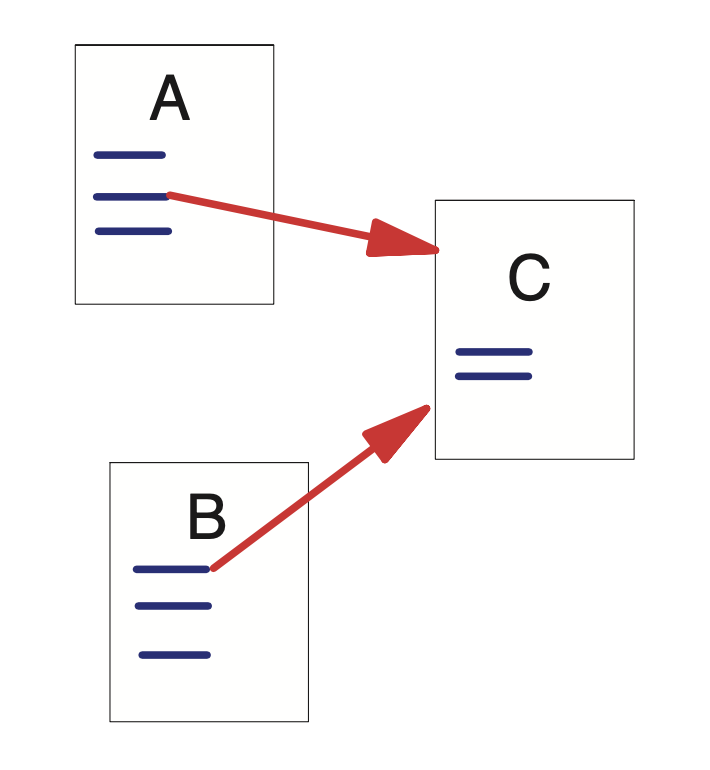
\includegraphics[width=0.2\textwidth]{pagerank-backref-small.png}
    \caption{A trivial page graph with two backreferences \autocite*[]{pagerank}}
    \label{kennan:fig:pagerank-backref-small}
\end{figure}
For instance, if we consider two websites $A$ and $B$,
both of which have outgoing links to $C$, we achive a simple graph
showing the \say{backreferences} of site $C$ as shown in Figure \ref{kennan:fig:pagerank-backref-small}.

If sites $A$ and $B$ are popular (highly ranked), $C$'s rank should be relatively
increased as a result of its backreference popularity. Likewise, if $A$ and $B$ are not
popular or notable, then $C$ is also unlikely to be popular without the presence of some other backreference.
In social networking literature, this notion of nodal popularity is commonly referred
to as \say{prestige}. This intuition forms the basis for PageRank.

To formalize this, if we consider a webpage $u$, a set of backreferences $B_u$ pointing to $u$,
and a set of forward references $F_u$ which are pointed to from $u$, then we can recursively define
the rank $R(u)$ of page $u$ as the sum of its backreference ranks \autocite*[]{pagerank},
\begin{equation}\label{kennan:eq:pagerank-simplified}
    R(u) = c \sum_{v \in B_u} \frac{R(v)}{|F_v|}
\end{equation}
where each backreference page divides its relative prestige across each of its outgoing links.
We can compute this for an entire graph by simply setting all ranks to \(R(u) = \frac{1}{|F_u|}\) initially
and then iterating with the recursive procedure until convergence.

\subsection{Handling Edge Cases}\label{kennan:sec:pagerank-extension}
\textit{(pardon the pun)}
The procedure described in Section \ref{kennan:sec:pagerank-intuition} is good, but can fail in a case where some set
of pages form a disconnected cycle, or a \say{sink}, and some other page points
to a page in this cycle, as demonstrated in Figure \ref{kennan:fig:pagerank-cycle}.
\begin{figure}[ht]
    \centering
    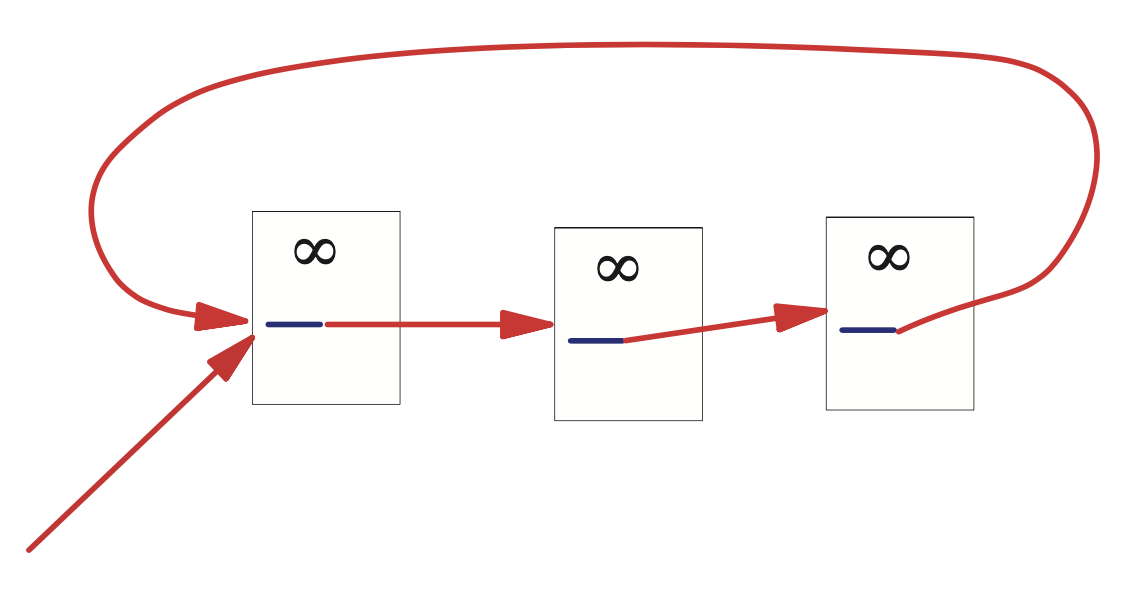
\includegraphics[width=0.5\textwidth]{pagerank-cycle.png}
    \caption{A page reference cycle \autocite*[]{pagerank}}
    \label{kennan:fig:pagerank-cycle}
\end{figure}
To resolve this case, we can add a \say{rank source} vector $E(u)$ to form a
modified rank equation \autocite*[]{pagerank}
\begin{equation}\label{kennan:eq:pagerank}
    R'(u) = c \sum_{v \in B_u} \frac{R'(v)}{|F_v|} + cE(u)
\end{equation}
where $c$ is maximized, and the $L_1$ norm of the rank is normalized such that $\lvert\lvert R' \rvert\rvert_1 = 1$.
In this instance, $E(u)$ acts as sort of decay term. We can analogously express the rank matrix $R'$ as
\begin{equation}\label{kennan:eq:pagerank-matrix}
    R' = c(AR' + E) = c(A + E \times \mathbf{1})R'
\end{equation}
(where $\mathbf{1}$ denotes a vector of all ones) which shows that the rank $R'$ is computable as
an eigenvector of the matrix $(A + E \times \mathbf{1})$.

\subsection{Computing PageRank}\label{kennan:sec:computing-pagerank}
To use the approach from Section \ref{kennan:sec:pagerank-extension}, we can initialize
an initial $R_0 := S$ for any vector $S$ over the set of pages. Then, we can perform
an iterative update by repeating
\begin{align}\label{kennan:eq:pagerank-power-procedure}
    R_{i+1} & \leftarrow AR_i                          \\
    d       & \leftarrow || R_i ||_1 - || R_{i+1} ||_1 \\
    R_{i+1} & \leftarrow R_i + dE                      \\
    \delta  & \leftarrow || R_{i+1} - R_i ||_1         \\
\end{align}
until convergence is achieved with $\delta \leq \epsilon$.

\section{LexRank: Technical Overview}\label{kennan:sec:lexrank}
LexRank \autocite*{lexrank-summarization} utilizes the PageRank algorithm in the context
of a document corpus in which we represent sentences as pages. With the basis laid out
in Section \ref{kennan:eq:pagerank}, we are able to establish several matrix of sentence
\say{centrality} within the context of a multi-document corpus within the
context of a multi-document corpus.

LexRank relies on the concept \textit{eigenvector centrality}, which is analogous to the rank vector as demonstrated
in Section \ref{kennan:sec:computing-pagerank}. In doing this, we can use the idea of a central sentence
being similar to many sentences to mimic the idea of prestige within the network, and use the same rank update
to compute sentence rankings iteratively.

\subsection{Constructing a Similarity Graph}\label{kennan:sec:lexrank-similarity-graph}
\begin{figure}[h]
  \centering
  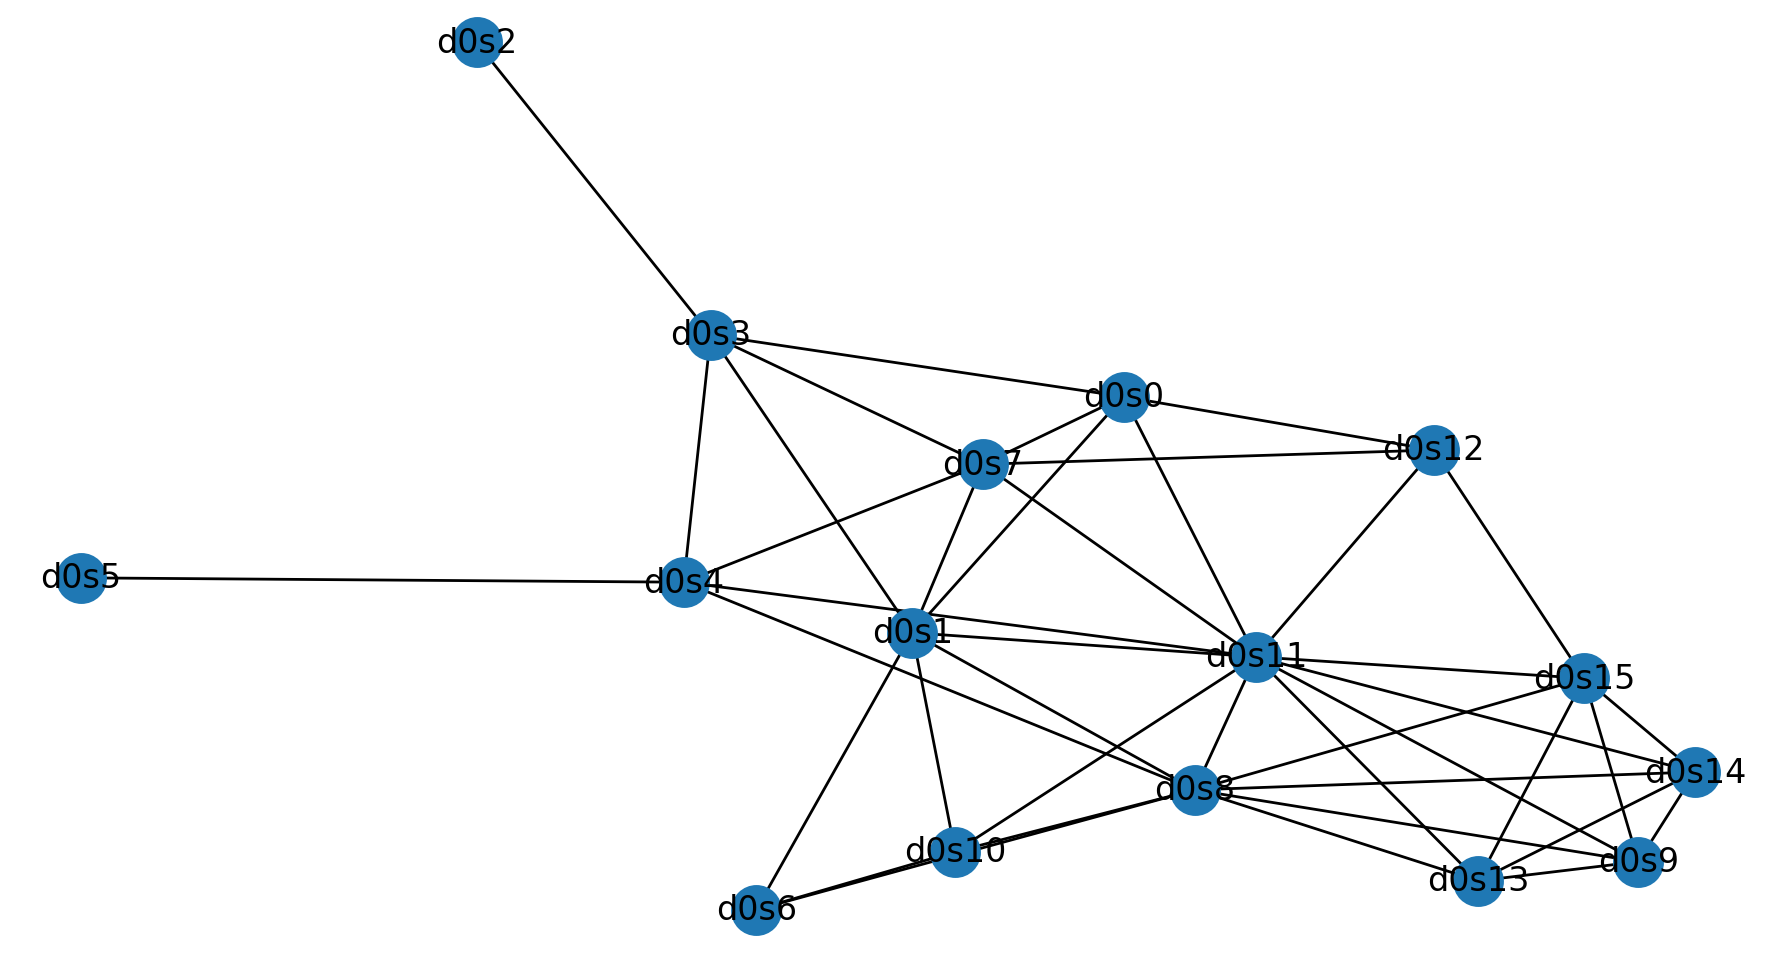
\includegraphics[width=0.6\textwidth]{lexrank-graph-.1.png}
  \caption{LexRank Continuous Similarity Graph}
  \label{kennan:fig:lexrank-similarity-graph}
\end{figure}
To formally model sentence salience via centrality, LexRank computes a similarity graph.
This computes a bag-of-words vector
for each sentence in a document corpus and connects sentence nodes according to
cosine similarity as in Equation \ref{kennan:eq:cosine-similarity}.
\begin{equation}\label{kennan:eq:cosine-similarity}
    cosine(x, y) =
    \frac{\sum_{w \in x,y} tf_{w,x} tf_{w, y} (idf_w)^2}
    {\sqrt{\sum_{x_i \in x} (tf_{x_i,x} idf_{x_i})^2 + \sum_{y_i \in y} (tf_{y_i,y} idf_{y_i})^2}}
\end{equation}
To leverage the results of this similarity, we can take the sentences within a document corpus as vertices, which are
connected with weights equal to the similarity values values. This forms the basis for \textbf{continuous eigenvector centrality}.
\textbf{continuous eigenvector centrality}, as shown in Figure \ref{kennan:fig:lexrank-similarity-graph}.
\begin{figure}[h]
  \centering
  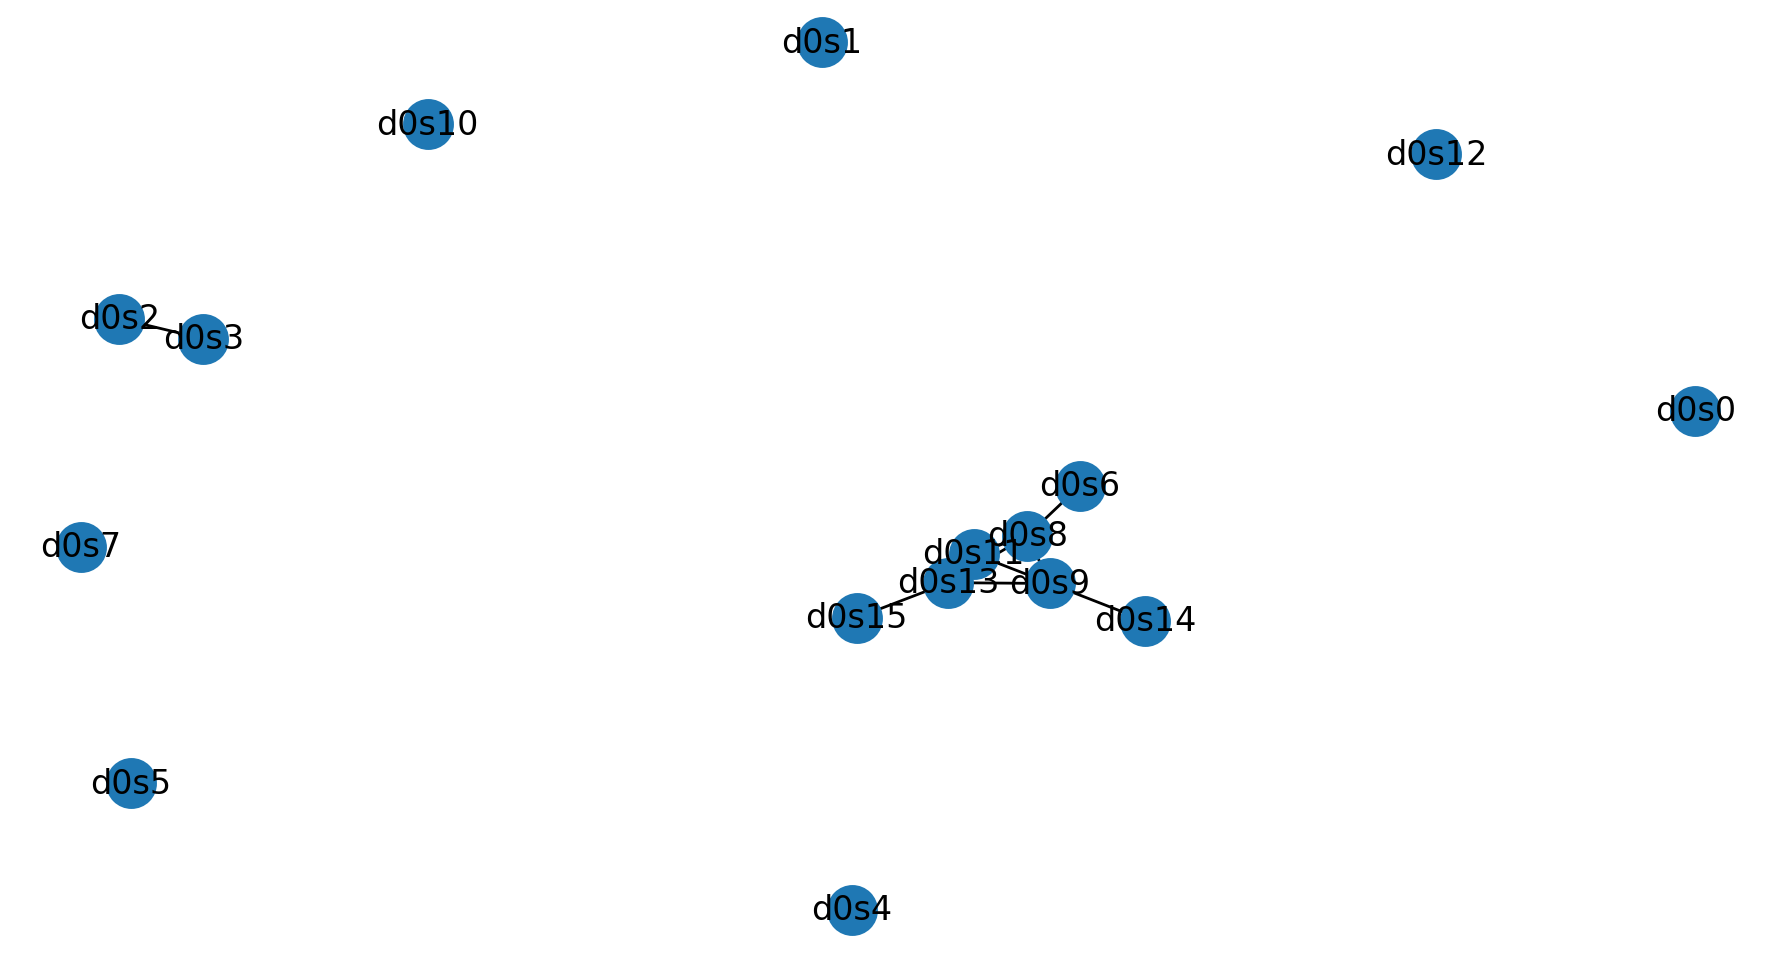
\includegraphics[width=0.6\textwidth]{lexrank-graph-.3.png}
  \caption{LexRank Discrete Similarity Graph, $t=0.3$}
  \label{kennan:fig:lexrank-discrete-similarity-graph}
\end{figure}
Alternatively, we can use an indicator matrix in which only sentences exceeding a
threshold similarity receive a connection, as demonstrated in Figure \ref{kennan:fig:lexrank-discrete-similarity-graph}.
This leads to a sparse representation with inherent lexical information loss, which we refer to as
\textbf{discrete eigenvector centrality}. We will discuss the impacts of this in a
later section.

\subsection{Power Method Ranking}\label{kennan:sec:power-method}
The Cosine Similarity graph described in Section \ref{kennan:sec:lexrank-similarity-graph} allows us to formalize
the rank equation much like PageRank,
\begin{equation}\label{kennan:eq:lexrank-equation}
    p(u) = \frac{d}{N} + (1 - d) \sum_{v \in adj(u)} \frac{p(v)}{d(v)}
\end{equation}
Analogously, we can express this in matrix form as a stochastic, irreducible markov transition
matrix to represent the LexRank vector with
\begin{equation}
    \mathbf{p} = \mathbf{B^Tp}
\end{equation}
where we can we can use the notion of a \say{random surfer} model as described in PageRank \autocite*[]{pagerank}.
In essence, the \say{random surfer} chooses an adjacent state with probability $(1 - d)$, or jumps to any state
in the graph at random with probability $d$, where this parameter acts as a damping factor $d$ for a modified matrix
\begin{equation}
    \mathbf{M} = [d\mathbf{U} + (1-d)\mathbf{B}]
\end{equation}
The eigenvector of this matrix forms the \textit{stationary distribution} of the stochastic Markov matrix $\mathbf{M}$.
With this basis, we can compute the stationary distribution $\mathbf{p}$ as
\begin{equation}\label{kennan:eq:power-method}
    \mathbf{p} = [d\mathbf{U} + (1-d)\mathbf{B}]^T\mathbf{p}
\end{equation}
according to the iterative procedure in Equation \ref{kennan:eq:pagerank-power-procedure}. Since the matrix is known
to be stochastic and irreducible, this method is guaranteed to achieve convergence.
and use this as our rank vector for choosing summary sentences.

\subsection{Document Penalization}\label{kennan:sec:document-penalty}
To extend the continuous form of the LexRank algorithm, we consider that although
LexRank is resistant to noisy documents, we can increase the
robustness of the algorithm by adding a penalty for sentences within the same document.

This means that where sentences $u, v$ would previously be joined with $cosine(u,v)$, we now
apply a penalty $0 < p < 1$, for which we can define a new edge weight function $w$, where we perform a linear
interpolation via the penalty term.
\begin{equation}\label{kennan:eq:document-penalty}
    w(uv) = \begin{cases}
        p \cdot cosine(uv) & \text{if u, v in same document} \\
        (1 - p) \cdot cosine(uv) & \text{otherwise}
    \end{cases}
\end{equation}

\section{Results and Analysis}
\end{document}